\documentclass[%
crop,%
tikz,%
convert={outext=.svg,command=\unexpanded{pdf2svg \infile\space../_static/\outfile}},%
multi=false%
]{standalone}%
\usepackage[utf8]{luainputenc}%
\usepackage[no-math]{fontspec}%
\defaultfontfeatures{%
    Numbers={OldStyle,Proportional},%
    Ligatures=TeX,%
    Extension=.ttf,%
}%
\setmainfont[%
UprightFont=*-Regular,%
ItalicFont=*-Italic,%
BoldFont=*-Bold,%
BoldItalicFont=*-BoldItalic,%
]{Raleway}%
\setsansfont[%
UprightFont=*-Regular,%
ItalicFont=*-Italic,%
BoldFont=*-Bold,%
BoldItalicFont=*-BoldItalic,%
]{Raleway}%
\usepackage[frenchmath]{mathastext}%
\usepackage{amsmath}%
\usepackage{amssymb}%
\usepackage{mathrsfs}%
\usepackage{mathtools}%
\usepackage{siunitx}%
\usepackage[siunitx]{circuitikz}%
\usetikzlibrary{calc,backgrounds,arrows.meta,patterns}%

\DeclareMathOperator{\sign}{sign}%

% Ensembles
\let\C\relax
\newcommand{\R}{\ensuremath{\mathbb{R}}} % Réel
\newcommand{\N}{\ensuremath{\mathbb{N}}} % Entiers naturels
% \newcommand{\C}{\ensuremath{\mathbb{C}}} % Complexes
\newcommand{\B}{\ensuremath{\mathscr{B}}} % Bus électriques
\newcommand{\Ch}{\ensuremath{\mathscr{C}}} % Charges
\renewcommand{\L}{\ensuremath{\mathscr{L}}} % Lignes
\renewcommand{\P}{\ensuremath{\mathscr{P}}} % Phases

% Phases
\newcommand{\arm}{\ensuremath{\mathrm{a}}}%
\newcommand{\brm}{\ensuremath{\mathrm{b}}}%
\newcommand{\crm}{\ensuremath{\mathrm{c}}}%
\newcommand{\nrm}{\ensuremath{\mathrm{n}}}%
\newcommand{\trm}{\ensuremath{\mathrm{t}}}%
\newcommand{\grm}{\ensuremath{\mathrm{g}}}%
\newcommand{\abrm}{\ensuremath{\mathrm{ab}}}%
\newcommand{\bcrm}{\ensuremath{\mathrm{bc}}}%
\newcommand{\carm}{\ensuremath{\mathrm{ca}}}%
\newcommand{\anrm}{\ensuremath{\mathrm{an}}}%
\newcommand{\bnrm}{\ensuremath{\mathrm{bn}}}%
\newcommand{\cnrm}{\ensuremath{\mathrm{cn}}}%
\newcommand{\atrm}{\ensuremath{\mathrm{at}}}%
\newcommand{\btrm}{\ensuremath{\mathrm{bt}}}%
\newcommand{\ctrm}{\ensuremath{\mathrm{ct}}}%
\newcommand{\ntrm}{\ensuremath{\mathrm{nt}}}%
\newcommand{\agrm}{\ensuremath{\mathrm{ag}}}%
\newcommand{\bgrm}{\ensuremath{\mathrm{bg}}}%
\newcommand{\cgrm}{\ensuremath{\mathrm{cg}}}%
\newcommand{\ngrm}{\ensuremath{\mathrm{ng}}}%
\newcommand{\abcrm}{\ensuremath{\mathrm{abc}}}%
\newcommand{\abcnrm}{\ensuremath{\mathrm{abcn}}}%

% Indices ou exposants
\newcommand{\cons}{\ensuremath{\mathrm{cons.}}}%
\renewcommand{\prod}{\ensuremath{\mathrm{prod.}}}%
\newcommand{\theo}{\ensuremath{\mathrm{th.}}}%
\newcommand{\const}{\ensuremath{\mathrm{const.}}}%

% Variables
\newcommand{\umax}{\ensuremath{U^{\max}}}%
\newcommand{\umaxnorm}{\ensuremath{U^{\max\,\text{norm.}}}}%
\newcommand{\umin}{\ensuremath{U^{\min}}}%
\newcommand{\uminnorm}{\ensuremath{U^{\min\,\text{norm.}}}}%
\newcommand{\unom}{\ensuremath{U^{\text{nom.}}}}%
\newcommand{\unomnorm}{\ensuremath{U^{\text{nom.}\,\text{norm.}}}}%
\newcommand{\uup}{\ensuremath{U^{\text{up}}}}%
\newcommand{\uupnorm}{\ensuremath{U^{\text{up}\,\text{norm.}}}}%
\newcommand{\uupprime}{\ensuremath{U^{\text{up}\,\prime}}}%
\newcommand{\udown}{\ensuremath{U^{\text{down}}}}%
\newcommand{\udownnorm}{\ensuremath{U^{\text{down}\,\text{norm.}}}}%
\newcommand{\udownprime}{\ensuremath{U^{\text{down}\,\prime}}}%
\newcommand{\smax}{\ensuremath{S^{\max}}}%
\newcommand{\pmax}{\ensuremath{P^{\max}}}%
\newcommand{\sproj}{\ensuremath{\underline{S^{\text{proj.}}}}}%
%

\begin{document}
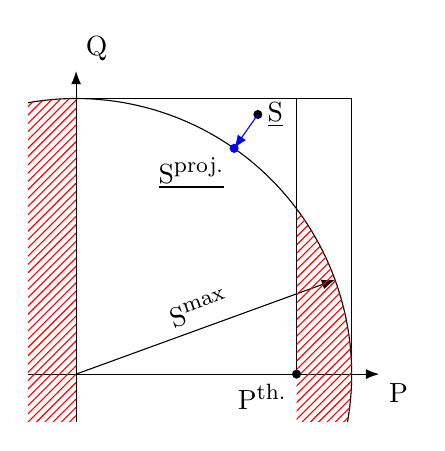
\begin{tikzpicture}[%
    show background rectangle,%
    tight background,%
    background rectangle/.style={fill=white}%
    ]
    % Styles
    \tikzset{fleche/.style={->, -{Latex}}}%
    \tikzset{interdit/.style={pattern=north east lines, pattern color=red}}%
    \tikzset{point/.pic={\filldraw[#1] (0,0) circle[radius=0.05];}, point/.default=black}%

    % Paramètres
    \pgfmathsetmacro{\r}{3.5}%
    \pgfmathsetmacro{\R}{1.1 * \r}%
    \pgfmathsetmacro{\pth}{0.8 * \r}%
    \pgfmathsetmacro{\angth}{acos(\pth/\r)}%
    \pgfmathsetmacro{\qth}{\r * sin(\angth)}%
    \pgfmathsetmacro{\startangle}{-10}%
    \pgfmathsetmacro{\endangle}{90-\startangle}%

    % Axes
    \pgfmathsetmacro{\tmp}{\r*cos(90-\startangle)};%
    \draw[fleche] (\tmp,0) -- (\R,0) node[below right] {$P$};%
    \pgfmathsetmacro{\tmp}{\r*sin(\startangle)};%
    \draw[fleche] (0,\tmp) -- (0,\R) node[above right] {$Q$};%

    % Circle
    \draw (\startangle:\r) arc[start angle=\startangle, end angle=\endangle, radius=\r];%
    \pgfmathsetmacro{\tmp}{\r*sin(\startangle)};%
    \pgfmathsetmacro{\tmpdeux}{\r*cos(\endangle)};%
    \pgfmathsetmacro{\tmptrois}{\r*sin(\endangle)};%
    \fill[interdit] (0,\tmp) -- (\tmpdeux,\tmp) -- (\tmpdeux,\tmptrois) arc[start angle=\endangle,
    end angle=90, radius=\r];%
    \draw[fleche] (0,0) -- (20:\r) node[above, midway, sloped] {$\smax$};%

    % Rectangle
    \draw (0,\r) -- (\r,\r) -- (\r,0);%

    % Theoretical power
    \draw (\pth,0) -- (\pth,\r) node[below left] at (\pth,0) {$P^{\theo}$};%
    \pgfmathsetmacro{\tmp}{\r*sin(\startangle)};%
    \fill[interdit] (\pth,\qth) arc[start angle=\angth, end angle=\startangle, radius=\r] --
    (\pth,\tmp);%

    % Point P^{\theo}
    \path (\pth,0) pic[pic type=point];%

    % Point outside of the circle
    \pgfmathsetmacro{\rayon}{1.15*\r}%
    \pgfmathsetmacro{\anglevaleur}{55}%
    \coordinate (S) at (\anglevaleur:\rayon);%

    \node[right] at (S) {$\underline{S}$};%
    \path (S) pic[pic type=point];%

    % Projection
    \coordinate (S correct) at (\anglevaleur:\r);%
    \draw[fleche, blue] (S) -- (S correct);%
    \path (S correct) pic {point=blue};%
    \node[below left] at (S correct) {$\underline{S^{\text{proj.}}}$};%
\end{tikzpicture}
\end{document}
% Local Variables:
% mode: latex
% TeX-engine: luatex
% TeX-source-correlate-method-active: synctex
% ispell-local-dictionary: "british"
% coding: utf-8
% LaTeX-indent-level: 4
% fill-column: 100
% End:
